% Overleaf: compile with pdfLaTeX. Self-contained (no external figures/bib files).
\documentclass[11pt,a4paper]{article}
\usepackage[margin=2.3cm]{geometry}
\usepackage[T1]{fontenc}
\usepackage[utf8]{inputenc}
\usepackage{lmodern}
\usepackage{microtype}
\usepackage{amsmath,amssymb,booktabs,tabularx,enumitem}
\usepackage{tikz}
\usetikzlibrary{positioning,arrows.meta}
\usepackage[colorlinks=true,linkcolor=blue!50!black,urlcolor=blue!60!black,citecolor=blue!50!black]{hyperref}
\newcommand{\file}[1]{\nolinkurl{#1}}
\setlength{\parindent}{0pt}
\setlength{\parskip}{5pt}
\setlength{\emergencystretch}{2em}
\renewcommand{\arraystretch}{1.15}

\title{Phase A Methodology:\\ A Causal Audit of Semantic Induction Heads on Single-hop In-context Relations}
\author{Daniella Simonovsky and Max Golubkov}
\date{Methodology specification --- September 2026}

\begin{document}
\maketitle

\section{Goal and Guiding Principles}
Ren et al.~\cite{ren} define \emph{semantic induction heads} (SIH) observationally, via the Relation Index (RI), and report correlations with ICL emergence --- with no interventions. Phase A asks: \textbf{do heads passing the SIH definition causally carry the model's single-hop in-context relation ability, and is the definition complete --- or are these heads the visible tip of a larger circuit?} (Phase B extends to two-hop composition.)

Four principles constrain everything below:
\begin{enumerate}[itemsep=1pt]
\item \textbf{Audit, not verification.} We measure the observational score \emph{and} the causal effect on \emph{all} $32\times32=1024$ heads, then compare the two rankings. Selecting heads by RI and testing only those would make the definition's misses invisible by construction.
\item \textbf{Definitional fidelity.} Parameters inside the SIH definition (notably the dominance threshold $\tau=2.2$) are kept exactly as published; we may not redesign the thing we are auditing. Deviations appear only as sensitivity analyses.
\item \textbf{Null-calibrated, pre-registered thresholds.} Every selection threshold is a \emph{rule} fixed before seeing results, calibrated against an explicit null distribution --- never a percentile of the empirical score distribution (which would ``select'' a fixed fraction of heads even under pure noise).
\item \textbf{Discovery / validation split.} All screening and selection uses the 89 discovery families (even family ids); the 87 validation families are touched only by the final faithfulness and generalization tests.
\end{enumerate}

\begin{figure}[ht]
\centering
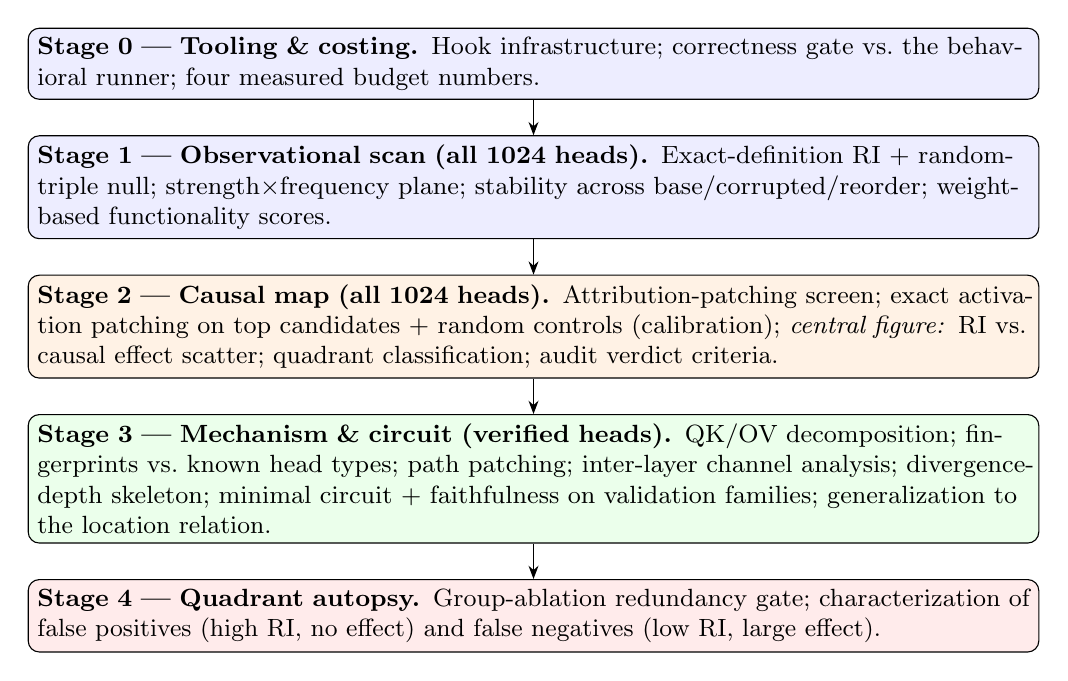
\begin{tikzpicture}[node distance=4.5mm,>=Stealth,
box/.style={draw,rounded corners,align=left,text width=12.6cm,minimum height=9mm,font=\small}]
\node[box,fill=blue!7]  (s0) {\textbf{Stage 0 — Tooling \& costing.} Hook infrastructure; correctness gate vs.\ the behavioral runner; four measured budget numbers.};
\node[box,below=of s0,fill=blue!7] (s1) {\textbf{Stage 1 — Observational scan (all 1024 heads).} Exact-definition RI + random-triple null; strength$\times$frequency plane; stability across base/corrupted/reorder; weight-based functionality scores.};
\node[box,below=of s1,fill=orange!10] (s2) {\textbf{Stage 2 — Causal map (all 1024 heads).} Attribution-patching screen; exact activation patching on top candidates + random controls (calibration); \emph{central figure:} RI vs.\ causal effect scatter; quadrant classification; audit verdict criteria.};
\node[box,below=of s2,fill=green!8] (s3) {\textbf{Stage 3 — Mechanism \& circuit (verified heads).} QK/OV decomposition; fingerprints vs.\ known head types; path patching; inter-layer channel analysis; divergence-depth skeleton; minimal circuit + faithfulness on validation families; generalization to the location relation.};
\node[box,below=of s3,fill=red!8] (s4) {\textbf{Stage 4 — Quadrant autopsy.} Group-ablation redundancy gate; characterization of false positives (high RI, no effect) and false negatives (low RI, large effect).};
\draw[->] (s0)--(s1); \draw[->] (s1)--(s2); \draw[->] (s2)--(s3); \draw[->] (s3)--(s4);
\end{tikzpicture}
\caption{Phase-A pipeline. Stages 1--2 are computed on \emph{every} head; stage 3 only on causally verified heads.}
\end{figure}

\section{Experimental Substrate}
\textbf{Model.} OLMo-2-1124-7B (base), revision pinned in \file{model_lock_olmo2.json}; fp16 across two 11--12\,GB GPUs. Pythia-6.9B retained as a contrast model for later comparisons.

\textbf{Data.} \file{pilot_v3/data_singlehop/singlehop_v1_*.jsonl}: 200 kinship families (relation \emph{mother-of} over fictitious names), each with three variants $\times$ two fact orders: \emph{base}; \emph{corrupted} --- the two answer-side names swapped inside the fact lines, so the former distractor becomes the correct answer while every mention count is unchanged and the two prompts are \textbf{token-aligned position-by-position} ($\le 6$ differing tokens); \emph{reorder} --- fact lines shuffled. Every fact line (demonstrations included) carries construction-time annotations: relation, head/tail entities, and their character spans --- the anchors RI needs, with no parser noise (an improvement over \cite{ren}'s spaCy/AGENDA annotation). A separate 50-family \emph{location} world (relation \emph{inside}) is reserved for the stage-3 generalization test.

\textbf{Working condition.} 4-shot with single-hop-only demonstrations (behavioral baseline: base $0.93$, corrupted $0.94$, reorder $0.89$ both-orders accuracy; working set of 176/200 families correct on base+corrupted in both orders). 0-shot is the secondary contrast. Demonstration sets are identical across all variants and orders of a family, so twins differ only in the test block.

\textbf{Primary metric for all interventions.} The candidate logit difference at the answer position,
\begin{equation}
M(x) \;=\; \mathrm{logit}\!\left(y_{\text{gold}}\mid x\right) - \mathrm{logit}\!\left(y_{\text{distractor}}\mid x\right),
\end{equation}
following the recommendations of \cite{bestpractices} (logit difference rather than probability or accuracy: linear in the final residual stream, sensitive, sign-interpretable). On a clean/corrupted twin the gold and distractor swap roles, so patching effects have a \emph{signed} prediction (the difference should flip toward the corrupted run's answer), not merely ``performance drops''.

\section{Stage 0 --- Tooling and Costing}
\textbf{What.} Stand up hook-based access to internal activations (read attention patterns and per-head outputs; write/replace head outputs mid-run) via TransformerLens \cite{tlens}, with raw PyTorch forward hooks on the HF model as fallback if the wrapper misbehaves on our sharded 2-GPU setup.

\textbf{Correctness gate.} Before any measurement: the hooked model must reproduce the behavioral runner's candidate scores on 20 prompts within numerical tolerance. No gate, no science.

\textbf{Why.} All later budgets depend on four numbers that cannot be reliably guessed for this hardware.

\begin{center}\small
\begin{tabular}{clp{7.6cm}}
\toprule
\# & Measurement & What it budgets \\
\midrule
1 & sec + GiB of a forward pass with attention caching & Stage-1 scan time ($\times$ \#prompts); cache is $L\,H\,n^2 \approx 32\cdot 32\cdot 350^2 \approx 1.3\times10^8$ values/prompt $\Rightarrow$ streaming policy \\
2 & sec of a full RI computation per prompt & Verifies the cheap order of operations (QK filter from cached attention first; OV vocabulary projection only for surviving (head, position) pairs at entity positions --- naively this stage costs $\sim$30 forwards/prompt) \\
3 & sec of one forward with a hook intervention & Unit price of exact patching (stage-2 verification budget) \\
4 & does a backward pass fit in GPU memory? & Gates attribution patching (needs $\partial M/\partial a$ for all sites); if not: 4-GPU jobs or memory-saving fallbacks \\
\bottomrule
\end{tabular}
\end{center}

\section{Stage 1 --- Observational Scan (all heads)}
\textbf{Implemented scope.} The final run, \file{stage1_v4_calibrated}, scanned all 1024 heads on 534 prompts: 89 working-set discovery families $\times$ three variants $\times$ two fact orders, with four ICL demonstrations. The model, dataset and behavioral working set were unchanged. Demonstrations were shared across variants and orders within each family. This section records the completed Stage-1 procedure; where it differs from the original plan elsewhere in this document, the specification below applies to Stage 1.

\subsection{Preflight and intervention-metric specification}
Raw PyTorch hooks on the HF model were used. Before scanning, the following checks were run:
\begin{enumerate}[itemsep=1pt]
\item Reproduce the behavioral runner's summed log-probability scores, scoring each complete candidate under its own continuation, on the first six selected prompts. Abort if no reference comparisons are available or the maximum drift is $\ge 0.05$.
\item Require inert hooks to preserve answer-position logits exactly and require attention capture to be available. Record the logit drift from the attention-capturing forward; no numerical acceptance threshold was imposed on that drift. Attention capture used the library's eager-attention fallback.
\item Require a self-patch of L16H0 on one prompt to change the intervention metric by less than $10^{-3}$.
\item Record exact twin-patching effects for eight early-layer heads on one aligned pair. This was a descriptive preview, not a structural-zero test or a full causal screen.
\end{enumerate}
The first three checks were mandatory. The six behavioral checks were rows from one family, not six independent families.

\textbf{Collision-free intervention metric.} For this run's intervention checks, tokenize each candidate continuation with a terminal period and find the first token at which the two continuations differ. If their common token prefix is $c$ and their first differing tokens are $g_k,d_k$, use
\begin{equation}
M(x)=\mathrm{logit}(g_k\mid x,c)-\mathrm{logit}(d_k\mid x,c).
\end{equation}
The prefix is empty when the first tokens already differ. Patches replace one head's slice of the input to the output projection at all \emph{original prompt} positions only; shared answer-prefix positions are recomputed. Tokenization-boundary inconsistencies or candidates without a differing token cause an error. Specifications were saved for all selected prompts, but shared-prefix families were not separately tested by the small GPU preflight. No new broad gradient-attribution or exact-patching scan was performed in Stage 1.

\subsection{Relation Index and multi-token adaptation}
For each annotated fact, $t_s$ is the child-name source and $t_o$ is the mother-name target. The source anchor is its \emph{last} token; the target's \emph{first} token is primary and its \emph{last} token is a sensitivity measure. Both scores are computed for every scored event, not only a subsample. Names remain multi-token: unlike the semantic-relation preprocessing in \cite{ren}, they are not replaced by single letters and function words are not removed.

For every fact and current position $j\ge\max(s,o_{\mathrm{last}})$:
\begin{enumerate}[itemsep=1pt]
\item \textbf{QK filter.} Using the model's captured attention, require
\begin{equation}
s=\arg\max_{k\le j} A^h_{j,k},\qquad
\frac{A^h_{j,s}}{\max_{k\ne s} A^h_{j,k}+10^{-9}}>\tau,\qquad \tau=2.2.
\end{equation}
Self-attention is allowed by this position range. This is an attention-dominance condition, not an activation-magnitude threshold.
\item \textbf{Embedding-level OV score.} Following the explicit projection in \cite{ren}, use the \emph{raw embedding of the current token}, $e_j=W_E[t_j]$:
\begin{equation}
p^{h,j}=\mathrm{softmax}(e_jW_V^hW_O^hW_U).
\end{equation}
Let $C_j$ contain the distinct token IDs visible through position $j$. Define
\begin{equation}
q_t^{h,j}=\max\left(0,p_t^{h,j}-\frac{1}{|C_j|}\sum_{u\in C_j}p_u^{h,j}\right),
\qquad a^{h,j}_{T}=\frac{q_{t_o}^{h,j}}{\sum_{u\in C_j}q_u^{h,j}}.
\end{equation}
Skip undefined scores, including a zero denominator. The target need not have the largest logit. This projection is not the head's actual attention-weighted contextual output and is not a causal logit change.
\end{enumerate}
OV projections are computed only after QK filtering and cached by head and current-token ID within a prompt.

\subsection{Frequency, strength and event-level audit}
Frequency is the number of QK passes divided by the number of eligible fact--position evaluations for that head. Strength is the mean RI over passes with defined scores. Neither quantity is behavioral accuracy or the fraction of prompts solved. Pooled statistics are retained per variant for comparison with the earlier run.

Every pass is also saved with its prompt/family, variant, fact, current position, block indices, token IDs, dominance ratio and available scores. Separate denominators retain zero-pass groups. Prompt text, token strings, offsets, annotations and demonstration IDs permit reconstruction of individual examples.

Analyses distinguish the \emph{fact's block} from the \emph{current position's block}: demo--demo, demo--test and test--test. The focused audit of L9H22 and L3H11 reports family coverage, conditional family means, repeated prefix/fact conditions, concrete events and comparisons with other visible tail names in the same individual block. Shared target/control tokens are flagged. Identical demonstration prefixes are not independent evidence; stability across variants alone is not evidence of semantic tracking. Corruption swaps answer-side names, so tracking is assessed against the actual annotations rather than assuming that the source must move.

\subsection{Descriptive controls and matched-target calibration}
\textbf{Historical pooled rule.} The scan retains a position-10 fake-target score and one uniformly sampled visible unique-token control per scored event. The earlier selection rule compared a head's pooled strength with the 99.9th percentile of random-token control means across heads having at least 50 scored events. This is retained as a historical descriptive comparison, \emph{not} as a calibrated per-head significance test; it does not justify an expected false-positive count. The saved small legacy null reservoir is not used for the new calibration.

\textbf{Additional calibration, specified before the final run.} This is a separate, narrower statistic, not a replacement for pooled RI. Include only test--test events whose fact target is one of the two answer candidates. Both candidate tail mentions must be fully visible, equal in token length at their fact occurrences, and distinct in first-token ID. Compare the true fact target's first-token score with the other candidate's score, holding the prompt, QK selection and normalization fixed. Exclusion reasons are recorded.

For each head and active family, average the true and alternative scores over matched events. Average these family means with equal family weight. Require at least 50 matched events across at least 10 families; otherwise report \emph{insufficient support}, not a negative finding.

Generate $B=100{,}000$ null draws (seed 20260913). Each draw uses one fair true/alternative swap per family, shared across all its events, variants, orders and heads. For observed family-averaged score $S_h$ and null scores $S_h^{(b)}$, compute the one-sided Monte Carlo value
\begin{equation}
p_h=\frac{1+\sum_{b=1}^{B}\mathbf{1}[S_h^{(b)}\ge S_h]}{B+1},
\end{equation}
with floating-point tie tolerance. Apply Holm correction across all 1024 heads, assigning unsupported heads $p=1$ internally. Selection requires adjusted $p\le0.05$ and a positive true-minus-alternative effect. Report support, effect, null mean/standard deviation, 95/99/99.9 percentiles and raw/adjusted $p$ values.

The interpretation assumes conditional exchangeability of true/alternative assignments under the null. Matching and family blocking do not prove that assumption; name preferences, QK selection and working-set selection can limit it. This is not a causal test. Only the first-target, matched-test statistic receives this calibration; demo and last-target scores remain descriptive. No bootstrap confidence intervals were computed.

\subsection{Dominance sensitivity, outputs and boundaries}
All dominance ratios satisfying $\arg\max A^h_{j,k}=s$ are collected \emph{before} thresholding, over every head, layer and eligible fact--position evaluation. Raw float32 values are stored on disk without a sampling cap. Exact empirical percentiles are computed globally and per layer. The global population is event-weighted and includes repeated demonstration prefixes, not family-balanced.

The final full-population 95th percentile was $\tau^*_{\mathrm{ours}}\approx4.482$. Since it exceeds 2.2, higher-threshold RI sensitivity can be computed by filtering saved events; this offline filtering was performed. No separate model run or matched-null recalibration at $\tau^*_{\mathrm{ours}}$ was performed. Other previously proposed threshold runs are not claimed as completed. Differences from 2.2 may reflect data, tokenization and sampling scope as well as the model.

\textbf{Execution and provenance.} One job ran the GPU scan, the two-head descriptive analysis and CPU-only calibration in sequence. Calibration reused saved scores without extra model forwards. Outputs include \file{head_stats.csv}, detailed compressed event/opportunity/prompt files, dominance values and percentiles, candidate analyses, and \file{null_calibration/}. Preflight results, model revision, input/code hashes, selected prompt IDs, metric specifications, seeds and calibration rules are recorded.

\textbf{Not implemented in this stage.} The originally proposed weight-only copying, token-matching and relation-word functionality scores were not computed. A contextual-residual OV variant and a broad causal head map were also not run. References elsewhere to these planned measurements do not imply completed Stage-1 results.

\section{Stage 2 --- Full Causal Map (all heads)}
\subsection{Attribution-patching screen}
Exact activation patching for all heads is infeasible ($1024 \times 178$ twin pairs $\approx 1.8\times10^5$ forwards). Instead, a first-order estimate of every head's patching effect is obtained from three passes per twin pair \cite{attrpatch}:
\begin{equation}
\widehat{\Delta M}_h \;=\; \big(a_h^{\text{corr}} - a_h^{\text{clean}}\big)^{\!\top} \frac{\partial M}{\partial a_h}\bigg|_{\text{clean}},
\end{equation}
where $a_h \in \mathbb{R}^{d_{\text{model}}}$ is head $h$'s output at the answer position. One clean forward, one corrupted forward, and one backward pass of $M$ yield $\widehat{\Delta M}_h$ for \emph{all} heads (and MLP layers, and all positions) simultaneously: $\approx 700$ forward-equivalents for the full discovery set.

\textbf{Known failure mode and mitigation.} The estimate is a first-order Taylor approximation; it under-estimates precisely where the path from the activation to the metric crosses saturated softmax plateaus --- i.e., it is biased \emph{against} sharply-attending heads, our most interesting candidates. Therefore:
\begin{enumerate}[itemsep=1pt]
\item \textbf{Calibration (pre-registered):} exact activation patching on the union of the top-25 heads by each ranking (RI, attribution, weight scores) plus 25 random heads, on 40 twin pairs. The exact-vs-estimate agreement (Spearman correlation) on this sample is itself a reported result; if $\rho < 0.7$, the screen is upgraded to integrated-gradients attribution (EAP-IG, $m{=}5$ interpolation steps \cite{eapig}) and re-calibrated.
\item Exact patching is always the measurement of record for any head individually discussed.
\end{enumerate}

\subsection{The central figure and the audit verdict}
The main deliverable: a scatter of all 1024 heads, $x$ = RI strength, $y$ = causal effect (calibrated estimate; exact where available), color = weight-based copy score. Threshold-free statistics reported: Spearman rank correlation between RI and causal effect over all heads; overlap curves (top-$k$ Jaccard).

\begin{figure}[ht]
\centering
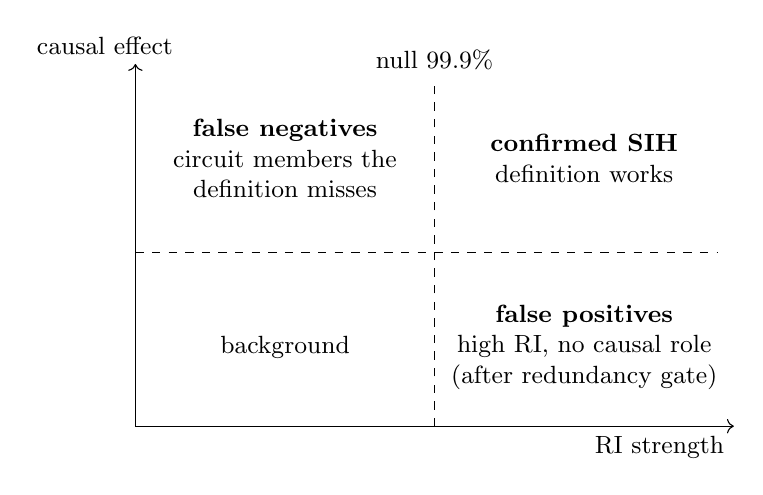
\begin{tikzpicture}[font=\small]
\draw[->] (0,0) -- (7.6,0) node[below left]{RI strength};
\draw[->] (0,0) -- (0,4.6) node[above left=0mm and -6mm]{causal effect};
\draw[dashed] (3.8,0) -- (3.8,4.4) node[above]{null 99.9\%};
\draw[dashed] (0,2.2) -- (7.4,2.2);
\node[align=center] at (5.7,3.4) {\textbf{confirmed SIH}\\definition works};
\node[align=center] at (1.9,3.4) {\textbf{false negatives}\\circuit members the\\definition misses};
\node[align=center] at (5.7,1.0) {\textbf{false positives}\\high RI, no causal role\\(after redundancy gate)};
\node[align=center] at (1.9,1.0) {background};
\end{tikzpicture}
\caption{Quadrant reading of the central scatter. Stage 4 characterizes the two off-diagonal quadrants.}
\end{figure}

\textbf{Pre-registered verdict criteria} (to be confirmed with the team before stage 2 runs):
the definition is judged \emph{sound} if RI-passing heads have systematically larger causal effects than layer-matched non-passing heads;
\emph{incomplete} if at least one head in the top decile of exact-patching effect lies below even the \emph{lenient} (99th-percentile) RI null threshold --- so that the incompleteness claim cannot be manufactured by our own strictness;
\emph{misleading} if the median causal effect of RI-passing heads does not exceed that of random heads.
These are not mutually exclusive (e.g., sound and incomplete). Note that the selection threshold never gates \emph{which heads are studied} --- the stage-2 causal map covers all 1024 heads unconditionally; the threshold only names the set attributed to the definition, and the primary quantitative claims are threshold-free (rank correlation, overlap curves).

\section{Stage 3 --- Mechanism and Circuit (verified heads only)}
Tools, in order of application:
\begin{enumerate}[itemsep=2pt]
\item \textbf{QK side --- edge-following score.} Using the fact anchors: attention mass from the answer position (and from the question-entity mention) to the correct fact's tail token, vs.\ positional controls; \emph{signed} version on corrupted twins (does attention move to the swapped source?).
\item \textbf{OV side --- what is written.} Project the head's actual output at the answer position to the vocabulary; verify it promotes the specific answer name; spectral copying check on the name subspace \cite{framework}.
\item \textbf{Fingerprints vs.\ known head types.} Standardized scores locate our heads in the existing taxonomy, answering ``new kind, or re-labeled known kind?'': prefix-matching and copying scores on random repeated sequences \cite{olsson}; retrieval-head score (fraction of copy events where the head's top attention sits on the copied token) \cite{retrieval}; function-vector mediation (does the head's mean output over relation prompts causally induce the relation zero-shot?) \cite{fv}. Deliverable: a head $\times$ fingerprint table.
\item \textbf{Path patching} \cite{ioi,patchguide}: which upstream components feed the verified heads' queries/keys/values, and which downstream components consume their output --- the head-vs-circuit question at edge resolution. Position-aware edges follow \cite{peap} given our templated prompts.
\item \textbf{Inter-layer channel content.} For each strong edge $A\!\to\!B$ found by path patching, SVD of the writer-reader interaction $W^A_{OV} W^B_{QK}$ to identify the low-rank communication subspace and interpret the message \cite{talking} --- the content-level refinement of \cite{framework}'s composition-strength norm.
\item \textbf{Divergence-depth skeleton.} Per layer $\ell$, the residual-stream distance at the answer position between the token-aligned twins, $d(\ell)=\|h^{\text{clean}}_\ell - h^{\text{corr}}_\ell\|$. The layer where $d$ jumps is where the swap's consequence reaches the answer position; all head-level findings must be consistent with this curve (a ``critical'' head above the completed divergence is a contradiction to explain). Nearly free from cached runs; comparison point to the layer-level analyses of parametric multi-hop work.
\item \textbf{Minimal circuit and faithfulness.} Define the circuit as the verified nodes + strong edges; run with everything else mean-ablated (means over discovery prompts); \textbf{pre-registered criterion:} the circuit must recover $\ge 80\%$ of the full model's clean--corrupted logit-difference gap on the \emph{validation} families. Completeness check: ablating the circuit from the full model must destroy the behavior.
\item \textbf{Generalization.} Repeat the RI scan + exact patching of the identified heads on the \emph{location} world: same heads $\Rightarrow$ general in-context relation machinery; disjoint heads $\Rightarrow$ relation-specific --- either outcome is a result.
\end{enumerate}

\section{Stage 4 --- Quadrant Autopsy}
\textbf{Gate first: group ablations.} A single-head zero effect does not prove irrelevance --- IOI-style backup heads activate when a primary head is removed \cite{ioi}. For each false-positive candidate: ablate jointly with all similarly-profiled heads and measure effect vs.\ coalition size. Only heads inert \emph{in coalition} are declared causally irrelevant; the effect-vs-coalition-size curve doubles as a quantitative distributedness measure.

\textbf{False positives (high RI, no causal role).} What are they instead? Weight fingerprints (stage 1), attention anatomy on our prompts (position? punctuation? relation word? recency?), and behavior on generic copying sequences. Deliverable: an alternative explanation for each head's high RI --- the empirical content behind ``the definition over-triggers''.

\textbf{False negatives (low RI, large effect).} What does the definition miss? Expected from our direct-path-blindness analysis: heads whose contribution is indirect (e.g., moving information between fact tokens rather than to the answer position), invisible to a metric that only reads the direct path to the logits. Characterized with the same tools; this quadrant, if populated, is the audit's sharpest finding.

Afterwards, as time permits: Phase B (two-hop composition, using the same verified single-hop circuit as the component inventory) and/or the checkpoint sweep.

\section{Summary of Pre-registered Decisions}
\begin{center}\small
\begin{tabular}{lp{9.6cm}}
\toprule
Item & Rule \\
\midrule
SIH definition parameters & $\tau=2.2$ exactly; sensitivity $\{1.5,3.0\}$ in appendix \\
Head selection threshold & 99.9th percentile of the random-triple null (per statistic); sensitivity at 99/99.5 \\
Screen quality gate & Spearman(exact, attribution) $\ge 0.7$ on the calibration sample, else upgrade to EAP-IG \\
Faithfulness criterion & $\ge 80\%$ recovery of the clean--corrupted logit-diff gap on validation families \\
Audit verdict definitions & sound / incomplete / misleading, as specified in \S5.2 \\
Selection data & discovery families only; validation families reserved for faithfulness + generalization \\
\bottomrule
\end{tabular}
\end{center}

\begin{thebibliography}{99}
\bibitem{ren} J.~Ren et al.\ (2024). \emph{Identifying Semantic Induction Heads to Understand In-Context Learning}. Findings of ACL. \url{https://aclanthology.org/2024.findings-acl.412/}
\bibitem{olsson} C.~Olsson et al.\ (2022). \emph{In-context Learning and Induction Heads}. Transformer Circuits Thread. \url{https://transformer-circuits.pub/2022/in-context-learning-and-induction-heads/index.html}
\bibitem{framework} N.~Elhage et al.\ (2021). \emph{A Mathematical Framework for Transformer Circuits}. Transformer Circuits Thread. \url{https://transformer-circuits.pub/2021/framework/index.html}
\bibitem{ioi} K.~Wang et al.\ (2022). \emph{Interpretability in the Wild: a Circuit for Indirect Object Identification in GPT-2 Small}. \url{https://arxiv.org/abs/2211.00593}
\bibitem{patchguide} S.~Heimersheim and N.~Nanda (2024). \emph{How to Use and Interpret Activation Patching}. \url{https://arxiv.org/abs/2404.15255}
\bibitem{bestpractices} F.~Zhang and N.~Nanda (2024). \emph{Towards Best Practices of Activation Patching in Language Models: Metrics and Methods}. ICLR. \url{https://arxiv.org/abs/2309.16042}
\bibitem{attrpatch} A.~Syed, C.~Rager, A.~Conmy (2023). \emph{Attribution Patching Outperforms Automated Circuit Discovery}. \url{https://arxiv.org/abs/2310.10348}
\bibitem{eapig} M.~Hanna, S.~Pezzelle, Y.~Belinkov (2024). \emph{Have Faith in Faithfulness: Going Beyond Circuit Overlap When Finding Model Mechanisms}. \url{https://arxiv.org/abs/2403.17806}
\bibitem{peap} T.~Haklay et al.\ (2025). \emph{Position-aware Automatic Circuit Discovery}. \url{https://arxiv.org/abs/2502.04577}
\bibitem{retrieval} W.~Wu et al.\ (2024). \emph{Retrieval Head Mechanistically Explains Long-Context Factuality}. \url{https://arxiv.org/abs/2404.15574}
\bibitem{fv} E.~Todd et al.\ (2024). \emph{Function Vectors in Large Language Models}. ICLR. \url{https://arxiv.org/abs/2310.15213}
\bibitem{maps} A.~Elhelo and M.~Geva (2024). \emph{Inferring Functionality of Attention Heads from their Parameters}. \url{https://arxiv.org/abs/2412.11965}
\bibitem{talking} J.~Merullo, C.~Eickhoff, E.~Pavlick (2024). \emph{Talking Heads: Understanding Inter-layer Communication in Transformer Language Models}. \url{https://arxiv.org/abs/2406.09519}
\bibitem{tlens} N.~Nanda and J.~Bloom. \emph{TransformerLens}. \url{https://github.com/TransformerLensOrg/TransformerLens}
\end{thebibliography}
\end{document}